\chapter{Deploying a Detector for \acp{EWFO} on a \ac{MAV}}


So far this work investigated the detection of \ac{EWFO} on a theoretical basis. A virtual dataset was created in which different network architectures were evaluated. In this chapter the application of a \ac{CNN} on an example \ac{MAV} is studied. The target system is the JeVois Smart Camera described in \Cref{background:jevois}. The detector is integrated in a control loop that is explained in detail in \Cref{background:system}. The on-board resources give severe limitations to the network that can be deployed. Furthermore, the global state estimation pipeline fuses data from different sensors and over time. Hence, it can be more important to have fast detections that are less accurate compared to slow but accurate detections. Therefore this chapter investigates the performance-accuracy trade-off in the example of the target system. The research question of this chapter is summarized in the following:

\begin{itemize}
	\item[RQ1] What are is the trade-off in terms of accuracy and inference time?
\end{itemize}

The limited resources on mobile devices makes the deployment of \acp{CNN} a challenging task. For example on pass of the state of the art \ac{CNN} ResNet101 contains of 11.3 billion floating point operations. Even assuming a powerful 2 GHz processor can perform 2 billion calculations per second it would still require almost 6 seconds for one network pass. Furthermore, a \acp{CPU} usually has to reload operands from the memory and cannot directly perform floating point multiplications. Hence, the actual forward pass would require even more time.

Therefore researchers address the reduction of inference time by reducing the number of operations. For example MobileNet and ShuffleNet aim to reduce the computations by addressing the expensive 3D convolutions. Other researchers aim to making the individual operations more efficient. This can be done by replacing floating point operations with integer operations hence quantizing the network.

In order to infer a layer in a \acp{CNN} kernels are convolved at multiple locations within one image. Thereby the same calculations are applied on various input data while the individual operations are independent of each other. Hence, theoretically the computations in one layer can be performed completely in parallel. The output of one layer can be stored similarly to the input image as a matrix. Computational platforms that exploit this fact are \acp{GPU} that have been adopted for Deep Learning applications from early on. In contrast to \acp{CPU} that are optimized to perform many different operations sequentially, \acp{GPU} typically consist of more cores and are optimized to perform the same operation on different data. While each individual core is typically slower than a single core in a \acp{CPU}, \acp{GPU} are much faster for applications that can be performed in parallel.

With a large enough \ac{GPU} it does not matter whether an operation is performed at an image of size 150x150 or 300x300 despite the actual computations increase by a factor of 4. However, such powerful \acp{GPU} require space and energy which is typically not available for small scale \acp{MAV}. The JeVois Smart Camera contains a MALI-400GPU with two cores and 408 Mhz each. Additionally it contains floating point registers and supports NEON operations. These are processor instructions that enable the efficient use of \acp{SIMD} operations.

The actual inference time of a network strongly depends on the computational platform, memory access times as well as the particular low level implementation. Hence, the number of computations within a network can only give a limited insight on the actual inference time. For example the \textit{TensorflowLite} framework allows the deployment of models created in \textit{tensorflow} on mobile processors. However, with this framework a the application of a single kernel on a 104x104 input volume takes 27.1 ms on the JeVois. In contrast, the same operation performed with the \textit{Darknet} framework that supports NEON operations takes only 5.07 ms. 

Therefore, the inference time of several layers is measured on the JeVois using the \textit{Darknet} framework. The results are displayed in \Cref{fig:bottleneck_jevois}. Each sample corresponds to the number of computations and their computational time in one layer. Dashed lines connect samples at the same resolution. It is apparent how the same amount of computations at a spatial resolution of 20x15 is more than 4 times faster than at a resolution of 160x120. 

\begin{figure}[hbtp]
	\centering
	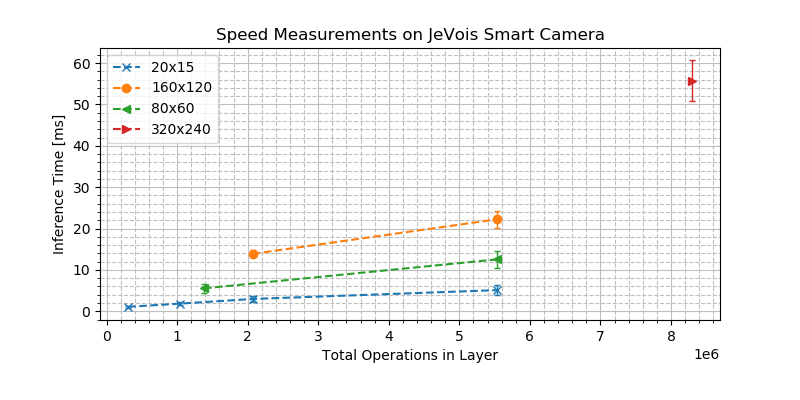
\includegraphics[width=0.8\textwidth]{fig/bottleneck_jevois}
	\caption{Inference Time of different layers on the JeVois. Each sample corresponds to the inference in a single layer. Dashed lines connect samples at the same resolution. It can be seen how an operation at a higher spatial resolution is significantly slower.}
	\label{fig:bottleneck_jevois}
\end{figure}

Hence, most speed can be gained when reducing the number of computations in the early layers where the spatial resolution is high. In \Cref{sec:object_detection} it could be seen that already a small amount of filters is enough to detect \acp{EWFO}. However, even evaluating 4 kernels at a resolution of 320x240 already takes 55 ms (\Cref{fig:bottleneck_jevois} red triangle). A total network of that size would require more than 200 ms and is thus too slow to be deployed in the control loop. Current research mostly addresses to reduce the computations when the convolved volumes are deep or the operations are performed on \acp{CPU} that do not support floating point operations. However, the bottleneck on the JeVois happens at small volumes and the hardware can perform floating point operations. Furthermore, \acp{EWFO} consist of thin elements that are spread over large parts of the image. Hence, we hypothesize that simply reducing the image resolution will lead to large drops in performance. An alternative is to increase the stride parameter in the early layers of the network. This reduces the number of locations at which the kernel is evaluated. \acp{EWFO} are sparse and spread over large parts of the image, while most of the image does not contain useful information. Hence, we hypothesize that increasing the stride parameter in the early layers will perform better than reducing the image resolution.

\section{Experiments}

In order to evaluate our hypotheses the network is trained with different architectures. Subsequently, performance and inference time on the JeVois are measured.

The JeVois supports aspect ratios of 4:3 and resolutions of 160x120, 320x240 and 640x480. Although, \ac{FCN} do not depend on the image resolution, the object appearance can change at lower image resolution. Hence, during training the images are scaled to 160x160 or 320x320 respectively. The anchor boxes are scaled in similar fashion. Finally, as the input image resolution decreases, the output grid size decreases by the same factor. This is not desirable as the output resolution should stay the same. Hence, when decreasing the input image to 160x160 we remove the last pooling layer such that the output grid stays at 20,20 or 10,10 respectively.

\section{Results}

\begin{figure}[hbtp]
	\centering
	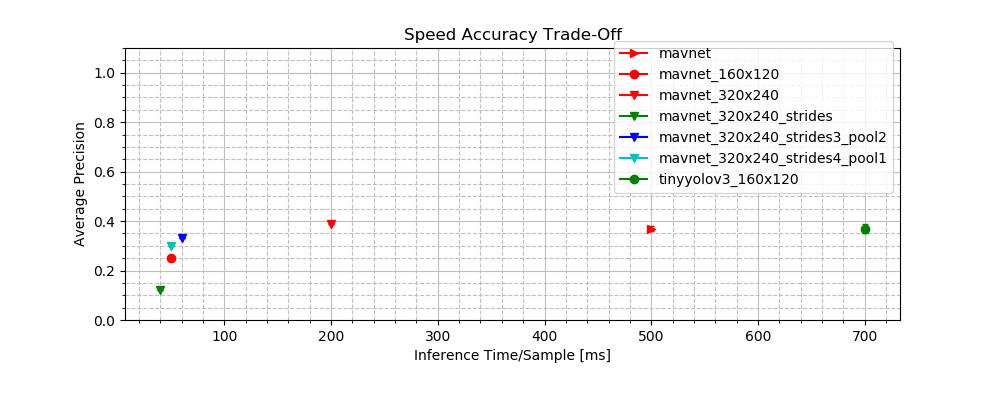
\includegraphics[width=0.8\textwidth]{fig/ap_speed_tradeoff}
	\caption{Inference Time of different layers on the JeVois. Each sample corresponds to a single layer. On the x-axis the total number of multiplications in that layer is displayed. It can be seen how an operation at a higher spatial resolution is significantly slower.}
	\label{fig:ap_speed_tradeoff}
\end{figure}

Due to their computational complexity deploying a \acp{CNN} on mobile devices is a challenging task

\section{Discussion}

\section{Conclusion}


In order to answer this question we measure the inference time of different model architectures. This enables us to investigate the bottlenecks and thus optimize the model architecture. The JeVois Smart Camera uses an aspect ratio of 4:3. Therefore we change the network resolution accordingly. The JeVois Smart Camera has only limited memory available. Using a network architecture that goes beyond the memory simply results in a system crash. For example our baseline network runs performs one network evaluation in 700 ms. This is at a resolution of 160x120.